%!TEX root = ../3dchapter.tex

\setchapterpreamble[u]{\margintoc}

\graphicspath{{csg_nef/}}
\renewcommand*{\thelesson}{4.2}

\chapter{Constructive solid geometry and Nef polyhedra}%
\label{chap:csg_nef}

% So far explicit, define

Until this lesson, we have only discussed data models that represent 3D geometries very \emph{explicitly}.
In other words, we have been specifying objects' shape through simple elements that have a direct geometric interpretation.
For instance, a tetrahedron's shape can be known by looking only at the coordinates of its four vertices, and a polyhedron's shape by looking at the set of its bounding polygons (which have a shape that is easily obtained from a list of vertices).
Even in a compact representation of a voxel grid, the geometry of a single voxel can be easily known based on a few simple parameters, such as: the absolute location and orientation of the voxel grid, the cell spacing along each axis, the order of the voxels in a linear encoding of the grid, and an index to identify the voxel in this encoding.

% Pros and cons

Since the elements in explicit representations can be interpreted easily, these kinds of explicit representations are usually the easiest for computers to process.
However, they also have disadvantages: since objects are often composed of many small elements, they can be very inefficient with space and can also make it difficult for people to define objects (either manually or automatically by writing software).
For instance, defining a shape that approximates a sphere using only polygons will require many small polygons to obtain a decent approximation, and defining the polygons to use (and their vertex coordinates) is not trivial.

% Define implicit

The alternative to the explicit approach is thus to use more \emph{implicit} representations\marginnote{implicit geometries}\index{implicit geometries}, in which objects are represented as \emph{sequences of operations on geometric primitives}.
Thus, the exact shape of the objects being represented is only known after performing the geometric operations, which can be rather complex.
However, the indirect approach makes it possible to use primitives that are better suited to a certain task, primitives that are easier to define, or simply fewer primitives overall.

\section{What is constructive solid geometry?}

Constructive solid geometry (CSG)\marginnote{constructive solid geometry}\index{constructive solid geometry}\marginnote{csg}\index{csg} is a general approach that combines many of techniques that are typically used with implicit representations, including primitive instancing, half-space intersections and Boolean set operations.
Most other data models that use implicit representations can thus be considered as variations of CSG, usually with more restrictions on the operations that can be performed or the primitives that can be used.

CSG represents objects as \emph{hierarchies of Boolean set operations} on other objects (\reffig{csg}).
A CSG object is thus a tree\marginnote{CSG tree}\index{CSG tree}, where each non-leaf node is a Boolean set operation on its children, and where the leaves are mathematical definitions of point sets, usually describing very simple objects.
In theory, arbitrary point sets can be used, although implementations usually limit them to some of the following:

\begin{figure}
\centering
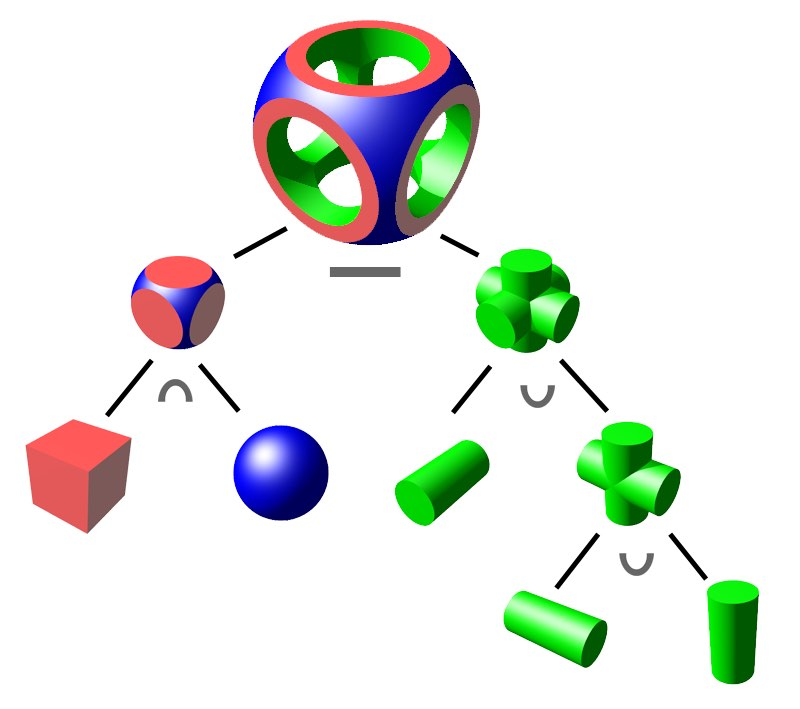
\includegraphics[width=0.7\linewidth]{figs/csg}
\caption{A CSG object represented as a tree of Boolean set operations on a sphere, a cube and three cylinders. From Wikimedia Commons.}%
\label{fig:csg}
\end{figure}

\begin{description}
\item[Primitive instancing] defines simple solids parametrically, such as a sphere based on a radius and the coordinates of its centre\marginnote{primitive instancing}\index{primitive instancing};
\item[Arbitrary polyhedra] defined using mesh data structures and boundary representation; and
\item[Half-spaces] (\reffig{halfspaces})\marginnote{half-space}\index{half-space} defined using a plane equation and a direction.
\end{description}

\begin{figure}
\centering
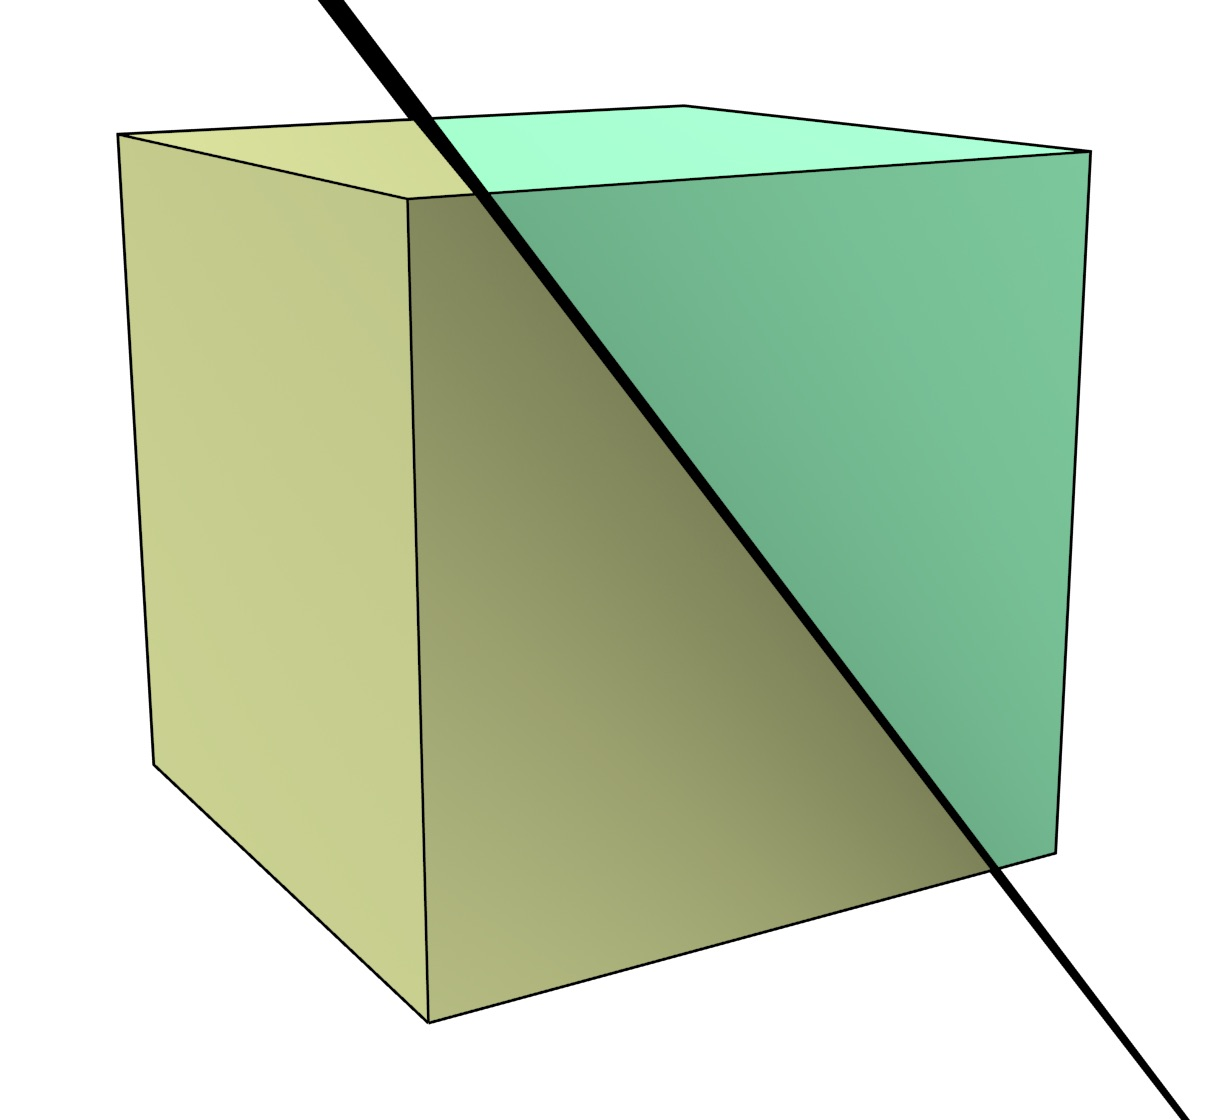
\includegraphics[width=0.3\linewidth]{figs/halfspaces}
\caption{A plane separates 3D space into two parts on either side of it. A plane and a direction can thus be used to specify the geometry of one of these halves, which forms an unbounded space on all directions except one.}%
\label{fig:halfspaces}
\end{figure}

The next section of the handout is a short summary of the mathematical background for this lesson, which consists of set theory, Boolean set operations and their mathematical notation.
Feel free to skip it if you are familiar with them.
In the next two sections, we look at how the two main elements of CSG work in theory: (i) the definition of simple objects as point sets, and (ii) how these elements can be combined using Boolean point set operations.
The final section covers Nef polyhedra, which are arguably the best known basis to implement CSG in practice.

\section{Background: set theory and Boolean set operations}

Set theory\marginnote{set theory}\index{set theory} is the branch of mathematics that studies \emph{sets}\marginnote{set}\index{set}, which are collections of abstract objects.
These objects can be anything, including other sets.

Set theory starts by considering the existence of a given domain of objects from which one may build sets, which is known as the \emph{universe set}\marginnote{universe set}\index{universe set} and denoted as \(\mathbb{U}\).
If an object \(a\) is part of a set \(\mathbb{X}\), it is denoted as \(a \in \mathbb{X}\), which is read as `\(a\) is an \emph{element}\marginnote{element of a set}\index{element of a set} of \(\mathbb{X}\)'.
If \(a\) is not part of a set \(\mathbb{X}\), it is denoted as \(a \notin \mathbb{X}\), which is read as `\(a\) is not an element of \(\mathbb{X}\)'.
By convention, lower case is usually used for simple elements and upper case for sets.

There are two common ways to describe the elements in a set, both using curly braces, \ie\ \{ and \}.
One way to do so is to list all the elements of the set one by one.
For instance, the set \(\left\{ 1,2,3 \right\}\) is the set containing \(1\), \(2\) and \(3\) as elements (and no others).
The other way to do so is to specify one or more rules that the elements of the set need to fulfil.
For instance, the set \(\{ x : x\)~\emph{is~a~prime~number}\(\}\) consists of all prime numbers.
It is read as `\(x\), such that \(x\) is a prime number'.

The order in which the elements in a set are defined does not matter.
That is, \(\left\{ 1,2,3 \right\}\) and \(\left\{ 3,2,1 \right\}\) are the same set.
The elements in a set are also unique, and duplicate items are ignored by convention.
That is, \(\left\{ 1,2,3 \right\}\) and \(\left\{ 1,2,3,2,1 \right\}\) are also the same set.

A set may contain an infinite number of elements (\eg\ as the prime number example above), or no elements at all, in which case it is a special set known as the \emph{null set}\marginnote{null set}\index{null set} or \emph{empty set}\marginnote{empty set}\index{empty set} and denoted as \(\{ \}\) or \(\emptyset\).
Other commonly used sets with a special notation and name are: the natural numbers (\(\mathbb{N}\)), the real numbers (\(\mathbb{R}\)), the rational numbers (\(\mathbb{Q}\)) and the integers (\(\mathbb{Z}\)).

In order to build more complex sets, the concepts and notation from mathematical logic are used, in particular \emph{propositional logic}\marginnote{propositional logic}\index{propositional logic}.
Propositional logic works with \emph{propositions}\marginnote{proposition}\index{proposition}, which are sentences that are either true or false, but not both.
These propositions might be altered and combined using various symbols expressing various notions, such as: \emph{and} (\(\wedge\)), \emph{or} (\(\vee\)), \emph{not} (\(\neg\)), \emph{implies} (\(\Rightarrow\)), \emph{is implied by} (\(\Leftarrow\)), \emph{if and only if} (\(\Leftrightarrow\)), \emph{for all} (\(\forall\)) and \emph{exists} (\(\exists\)).
These symbols correspond to their names.
For instance, \(a \wedge b\) is true only when both \(a\) and \(b\) are true, \(a \vee b\) is true when \(a\) or \(b\) are true (or both), and \(\neg a\) is true when \(a\) is false.

Using these concepts it is possible to state relationships between sets\marginnote{relationship between sets}\index{relationship between sets}.
For instance, we can define that \(\mathbb{A}\) and \(\mathbb{B}\) are equal (\(\mathbb{A} = \mathbb{B}\)) when an element is in \(\mathbb{A}\) if and only if it is also in \(\mathbb{B}\), which can be denoted as \(\forall x : x \in \mathbb{A} \Leftrightarrow x \in \mathbb{B}\).
A set \(\mathbb{A}\) is called a subset\marginnote{subset}\index{subset} of a set \(\mathbb{B}\) (\(\mathbb{A} \subseteq \mathbb{B}\)), or \(\mathbb{B}\) is a superset\marginnote{superset}\index{superset} of \(\mathbb{A}\) (\(\mathbb{B} \supseteq \mathbb{A}\)), when if an element is in \(\mathbb{A}\) then it is also in \(\mathbb{B}\), denoted as \(\forall x : x \in \mathbb{A} \Rightarrow x \in \mathbb{B}\).
If \(\mathbb{A} \subseteq \mathbb{B}\) but \(\mathbb{A} \neq \mathbb{B}\), \ie\ there is at least one extra element in \(\mathbb{B}\), then \(\mathbb{A}\) is a proper subset\marginnote{proper subset}\index{proper subset} of \(\mathbb{B}\) (\(\mathbb{A} \subset \mathbb{B}\)), or alternatively \(\mathbb{B}\) is a proper superset\marginnote{proper superset}\index{proper superset} of \(\mathbb{A}\) (\(\mathbb{B} \supset \mathbb{A}\)).
Note that these relationships are akin to `less than' (\(<\)), `less or equal than' (\(\leq\)), `equal to' (\(=\)), `greater or equal than' (\(\geq\)), and `greater than' (\(>\)) for numbers.

It is also possible to use propositional logic to create new sets by defining certain operations between sets, in particular \emph{Boolean set operations}\marginnote{Boolean set operation}\index{Boolean set operation}, consisting of intersection, union, difference and complement.
The intersection\marginnote{intersection}\index{intersection} of the sets \(\mathbb{A}\) and \(\mathbb{B}\), denoted as \(\mathbb{A} \cap \mathbb{B}\), consists of all the elements that are both in \(\mathbb{A}\) and in \(\mathbb{B}\), \ie\ \(\mathbb{A} \cap \mathbb{B} = \left\{ x : x \in \mathbb{A} \wedge x \in \mathbb{B} \right\}\).
The union\marginnote{union}\index{union} of the sets \(\mathbb{A}\) and \(\mathbb{B}\), denoted as \(\mathbb{A} \cup \mathbb{B}\), consists of all the elements that are either in \(\mathbb{A}\) or in \(\mathbb{B}\), \ie\ \(\mathbb{A} \cup \mathbb{B} = \left\{ x : x \in \mathbb{A} \vee x \in \mathbb{B} \right\}\).
The difference\marginnote{difference}\index{difference} between sets \(\mathbb{A}\) and \(\mathbb{B}\), denoted as \(\mathbb{A} - \mathbb{B}\), consists of all the elements that are in \(\mathbb{A}\) but not in \(\mathbb{B}\), \ie\ \(\mathbb{A} - \mathbb{B} = \left\{ x : x \in \mathbb{A} \wedge x \notin \mathbb{B} \right\}\).
The complement\marginnote{complement}\index{complement} of a set \(\mathbb{A}\), denoted as \(\neg \mathbb{A}\), consists of all the elements that are in the universe set but are not in \(\mathbb{A}\), \ie\ \(\neg \mathbb{A} = \left\{ x : x \in \mathbb{U} \wedge x \notin \mathbb{A} \right\}\).

Apart from sets, it is also possible to consider \emph{tuples}\marginnote{tuple}\index{tuple} of elements, which are sequences of ordered elements.
A tuple containing exactly two elements is known as a \emph{pair}\marginnote{pair}\index{pair}, one containing three elements is a \emph{treble}\marginnote{treble}\index{treble} and one containing \(n\) elements is an \(n\)-tuple.
Tuples are usually denoted using parenthesis, \ie\ (\ and~).

A common operation that generates tuples is the Cartesian product.
The Cartesian product\marginnote{Cartesian product}\index{Cartesian product} of sets \(\mathbb{A}\) and \(\mathbb{B}\), denoted as \(\mathbb{A} \times \mathbb{B}\), is defined as \(\left\{ (a,b) : a \in \mathbb{A} \wedge b \in \mathbb{B} \right\}\).
In other words, it is a set of pairs, where the first element of a pair is an element of \(\mathbb{A}\) and the second element of the pair is an element of \(\mathbb{B}\).
This can be generalised to more than two sets, such that the \(n\)-fold Cartesian product of \(n\) sets is an \(n\)-tuple.
The \(n\)-fold Cartesian product of a set \(\mathbb{A}\) with itself, \ie\ \(\mathbb{A} \times \mathbb{A} \times \cdots \mathbb{A}\), is denoted as \(\mathbb{A}^n\).

\section{Defining objects using point set geometry}%
\label{sec:ps}

Point set geometry applies the notions of set theory to define the geometry of objects as sets of points.
The usual definition maps 1D space (\ie\ the line) to the set of real numbers (\ie\ \(\mathbb{R}\)), and so 2D space (\ie\ the plane) is \(\mathbb{R}^2\) and 3D space is \(\mathbb{R}^3\).

Individual points in 2D and 3D space can be considered as elements of \(\mathbb{R}^2\) and \(\mathbb{R}^3\).
For instance, we can denote a point \(p\) in 2D space as \(p \in \mathbb{R}^2\) or in 3D space as \(p \in \mathbb{R}^3\).
Note that this notation perfectly matches the way in which points are usually defined based on their coordinates.
For example, by stating \(p = (x, y, z) \in \mathbb{R}^3\), we simply mean that \(x,y,z \in \mathbb{R} \), \ie\ that \(x\), \(y\) and \(z\) are arbitrary real numbers.

Based on these definitions, we can then define sets that describe specific geometric objects.
For instance, we can start by considering how any point \(p\) between two points \(p_1\) and \(p_2\) at different locations can be obtained as a sort of weighted average of \(p_1\) and \(p_2\), where the relative weight of the two points tell us that we're closer to one point than to another.
If we put this into an equation, we get:

\begin{equation}
p = \frac{a p_1 + b p_2}{a+b}.
\end{equation}

Note that we divide everything by \(a+b\) to make sure that the weights add up to one.
Also, note it is possible to use negative weights to get points that are on the line that passes through \(a\) and \(b\) but not between \(a\) and \(b\).
Expanding on this, the line \(L\)\marginnote{point set equation of a line}\index{point set equation of a line} passing through \(p_1\) and \(p_2\) is defined by considering all possible values of \(a\) and \(b\).
That is:

\begin{equation}
\label{eq:line}
L = \left\{ \frac{a p_1 + b p_2}{a+b} : a,b \in \mathbb{R} \right\}.
\end{equation}

In the case of a line, we can get rid of one parameter by substituting \(t = a/(a+b)\), which would yield \(L = \left\{ t p_1 + (1-t) p_2 : t \in \mathbb{R} \right\} \).
Note how at \(t = 0\) we get \(p_2\), at \(t = 1\) we get \(p_1\), and when \(0 < t < 1\) we get the line segment between \(p_1\) and \(p_2\).
Note also how this definition of a line works both in 2D and 3D.

Generalising from \refeq{line}, we can also define a similar equation for a plane \(P\)\marginnote{point set equation of a plane}\index{point set equation of a plane} from three non-collinear points \(p_1\), \(p_2\) and \(p_3\) as:

\begin{equation}
P = \left\{ \frac{a p_1 + b p_2 + c p_3}{a+b+c} : a,b,c \in \mathbb{R} \right\}.
\end{equation}

In 3D, if we substitute the equality (\(=\)) of the previous equation for a strict inequality (\(<\) or \(>\)), we get instead an equation to represent the half-spaces\marginnote{point set equation of a half-space}\index{point set equation of a half-space} respectively below and above the plane (such as those previously shown in \reffig{halfspaces}).
An equation of this form is typically stored in the leaves of a CSG tree, \eg\ as the three non-collinear points in the equation above, or as the coefficients of an equation of the form \(ax + by + cz + d = 0 \), plus a direction to specify which half-space to use.

For the sake of uniformity and ease of processing, many CSG implementations only use half-spaces.
However, several simple axis-aligned 3D solids also have easy point set definitions that can be used to store them as primitives based on a few parameters, including:

\begin{description}
\item[balls] \ie\ the space inside a sphere\marginnote{point set equation of a ball}\index{point set equation of a ball}, which can be defined as \( (x-c_x)^2 + (y-c_y)^2 + (z-c_z)^2 < r^2\), where \(r\) is the radius and \(c = (c_x, c_y, c_z)\) is the centre;
\item[ellipsoid interiors] defined\marginnote{point set equation of an ellipsoid}\index{point set equation of an ellipsoid} as \( \frac{(x-c_x)^2}{a^2} + \frac{(y-c_y)^2}{b^2} + \frac{(z-c_z)^2}{c^2} < 1 \), where \(a\), \(b\) and \(c\) are half the lengths of each axis, and \(c = (c_x, c_y, c_z)\) is the centre; and
\item[cuboid interiors] \ie\ box-shaped objects\marginnote{point set equation of a cuboid}\index{point set equation of a cuboid}, which can be defined using intervals for the minimum and maximum values it has along each axis, \ie\ \( x_\mathrm{min} < x < x_\mathrm{max} \wedge y_\mathrm{min} < y < y_\mathrm{max} \wedge z_\mathrm{min} < z < z_\mathrm{max} \); and
\item[cylinder interiors] by\marginnote{point set equation of a cylinder}\index{point set equation of a cylinder} checking whether a point lies within a radius for two axes, and within an interval for the third.
\end{description}

Other common objects are more general versions of these objects, such as parallelepipeds, (truncated) cones, etc.
As for non-axis aligned simple solids, they can be supported by special nodes in the CSG tree that represent geometric transformations by their parameters (rather than Boolean point set operations), such as translations, rotations and scaling, or more general ones like affine transformations or arbitrary transformation matrices by storing their elements one by one.

\section{Boolean point set operations}
\label{sec:psetops}

In order to create objects other than those directly added to an implementation (\ie\ half-spaces and possibly some geometric shapes), CSG relies on Boolean point set operations (\reffig{boolean}).
Arbitrary polyhedra can be represented in this way by first splitting them into convex parts\marginnote{convex decomposition}\index{convex decomposition} (which might require Steiner vertices), and then representing the convex parts as intersections of half-spaces (one per face).
These operations, which are located in the non-leaf nodes of the CSG tree, combine the geometry of the point sets described by their children (using the methods described in the previous section).

\begin{figure}
\centering
\begin{subfigure}[b]{0.5\linewidth}
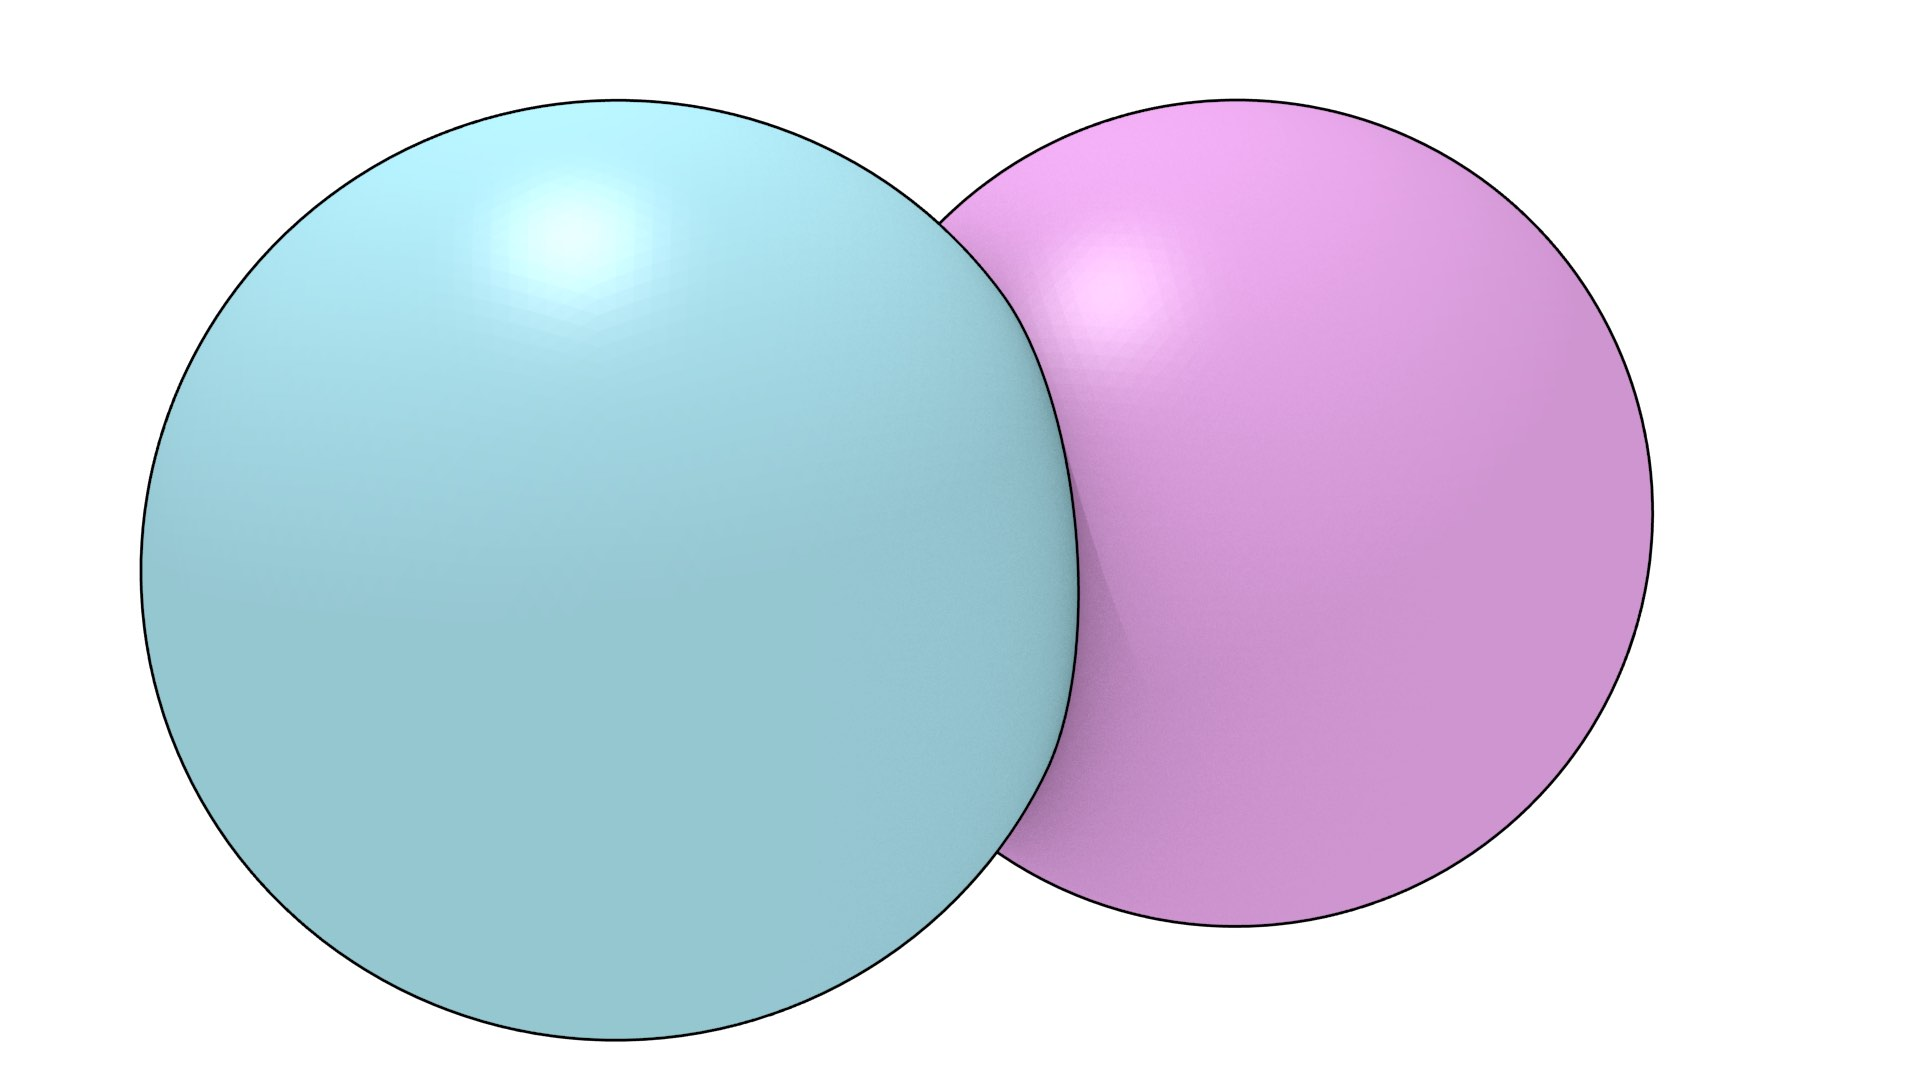
\includegraphics[width=\linewidth]{figs/boolean}
\caption{}%
\label{subfig:boolean}
\end{subfigure}%
\begin{subfigure}[b]{0.5\linewidth}
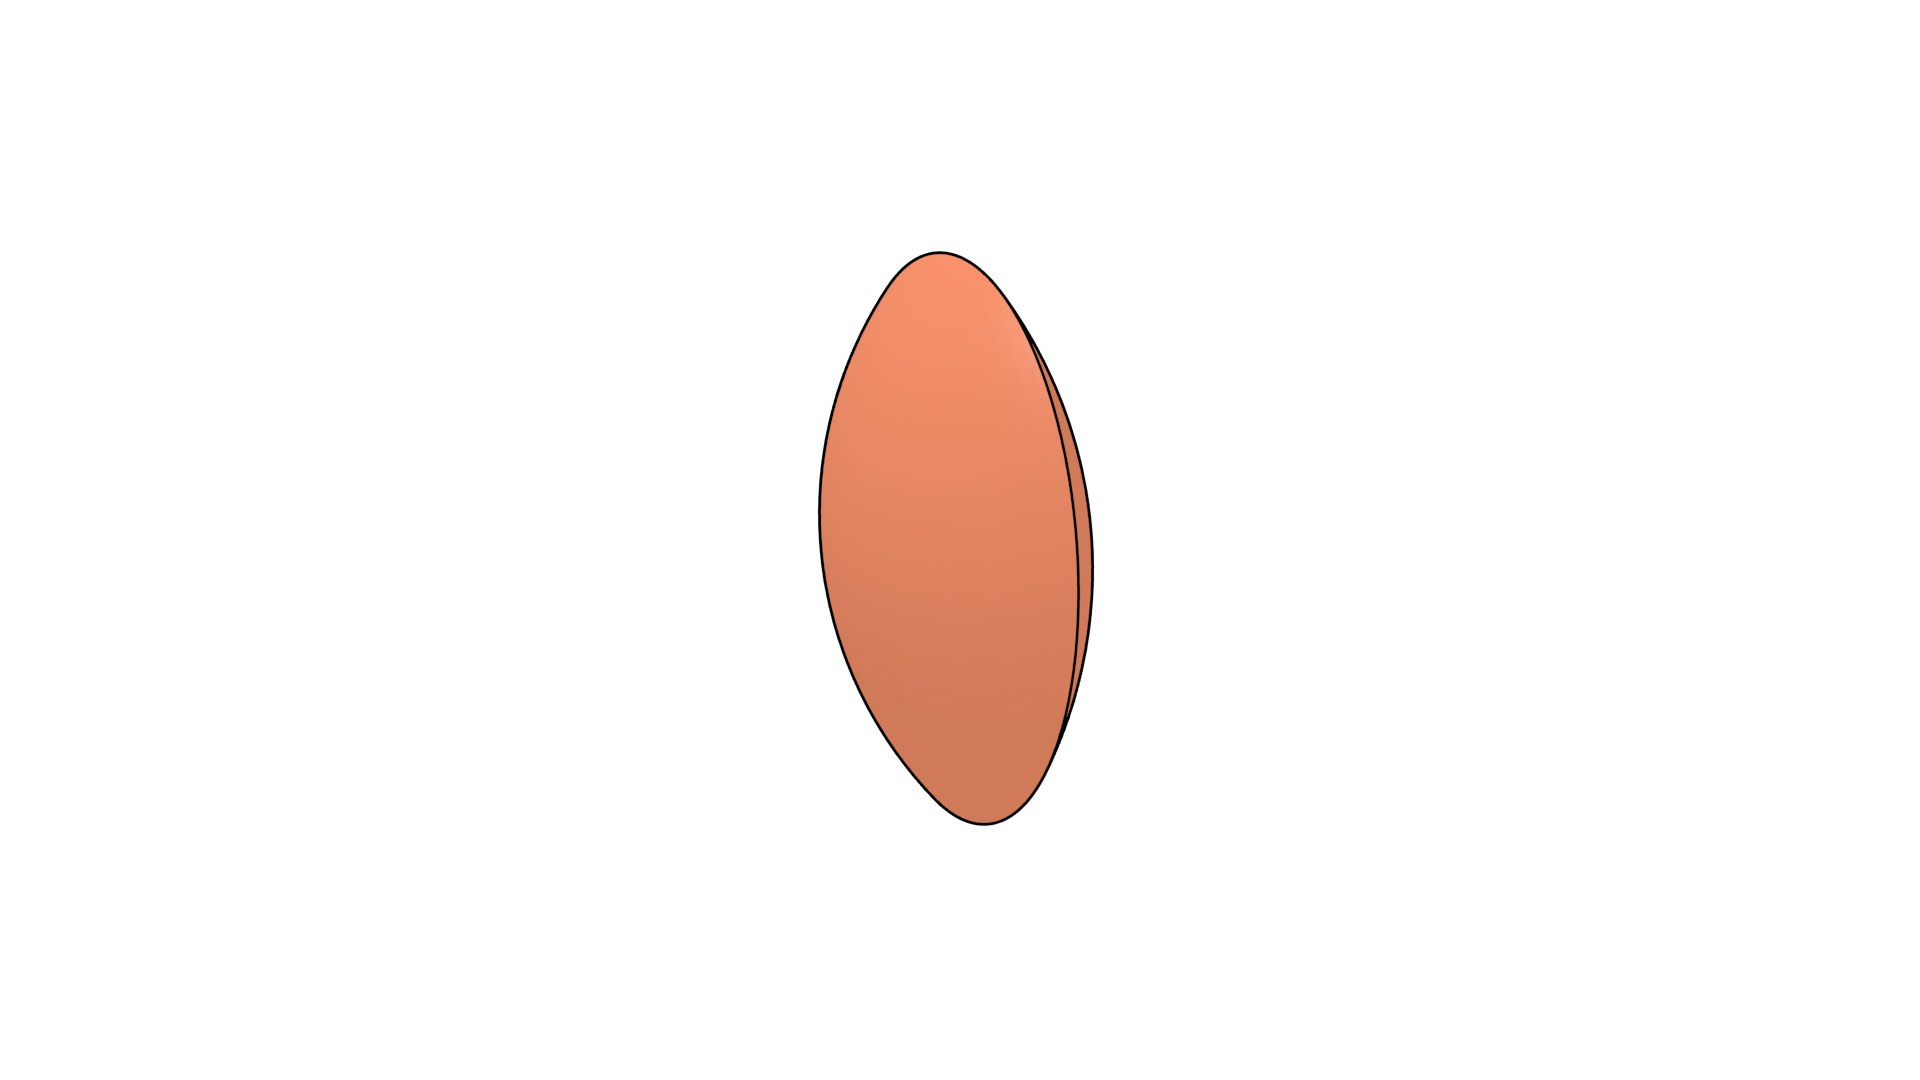
\includegraphics[width=\linewidth]{figs/boolean-intersection}
\caption{}%
\label{subfig:boolean-intersection}
\end{subfigure}\\
\begin{subfigure}[b]{0.5\linewidth}
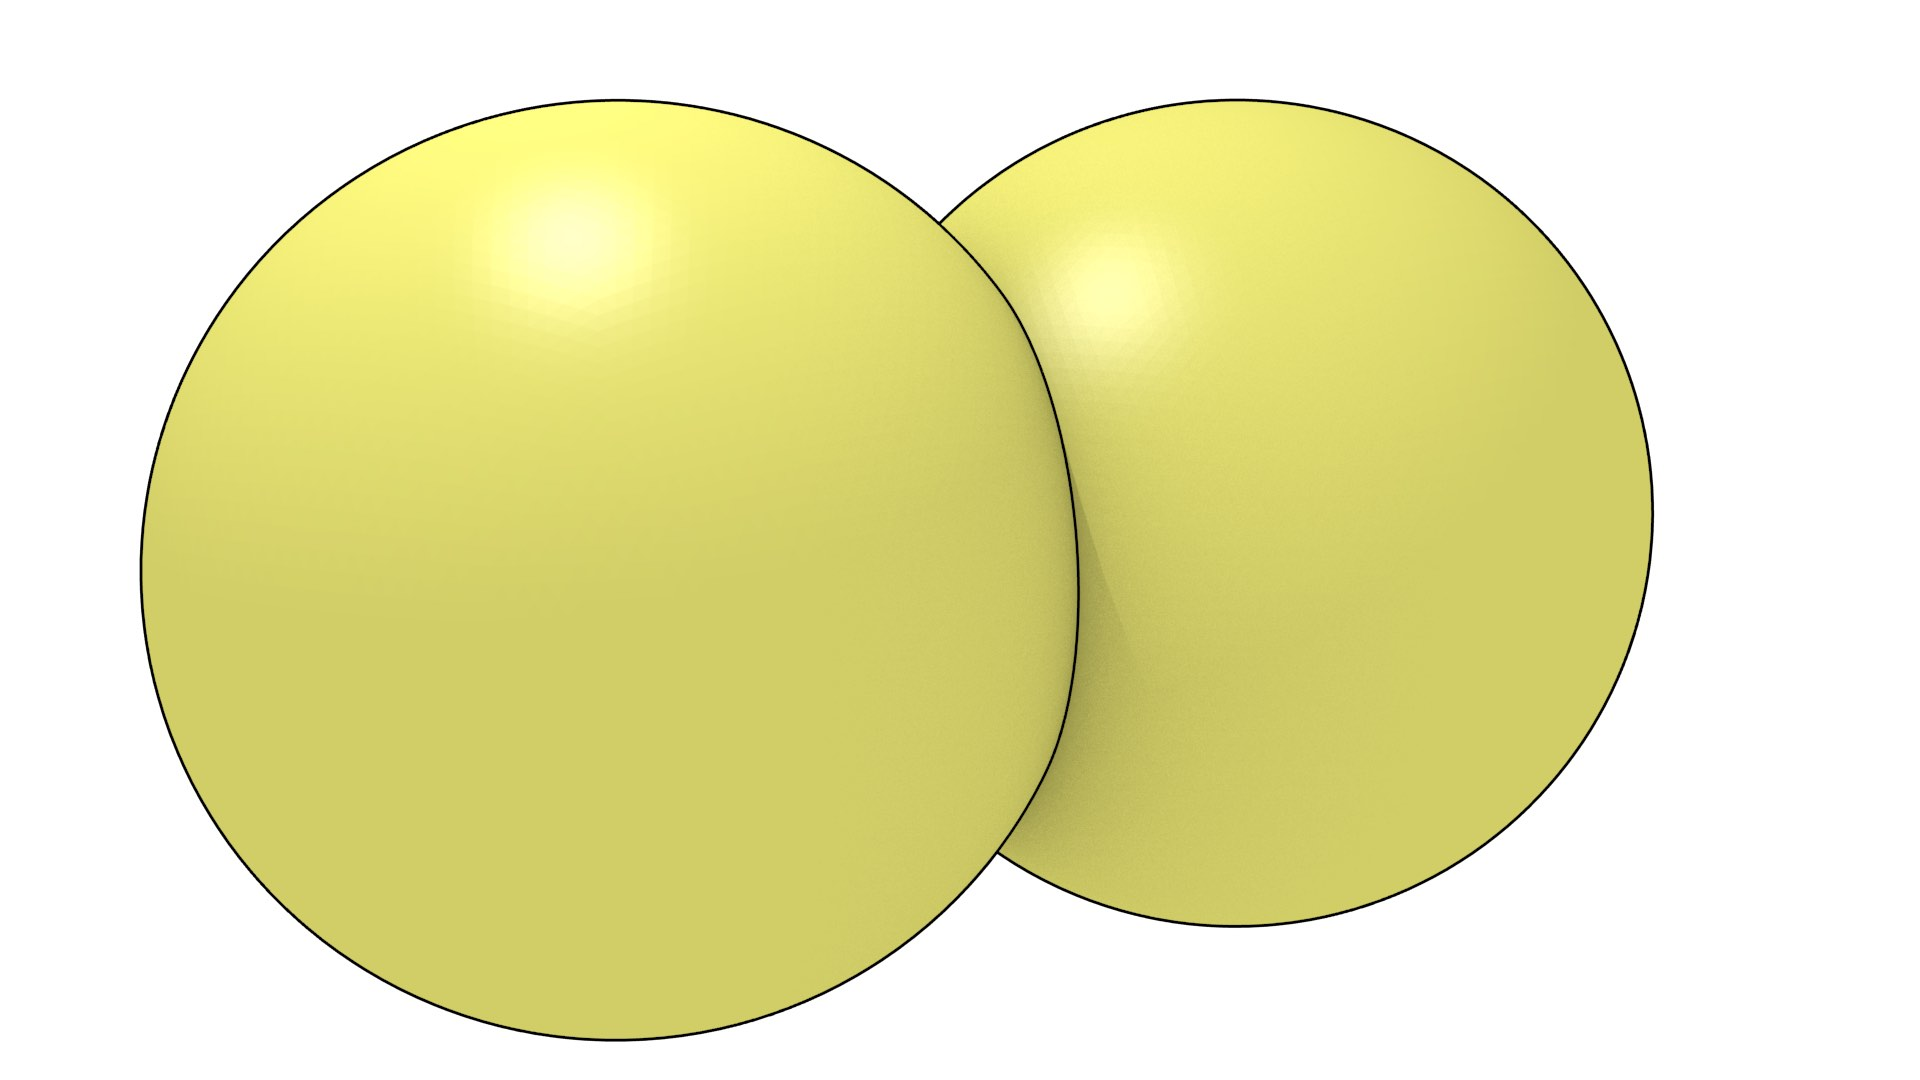
\includegraphics[width=\linewidth]{figs/boolean-union}
\caption{}%
\label{subfig:boolean-union}
\end{subfigure}%
\begin{subfigure}[b]{0.5\linewidth}
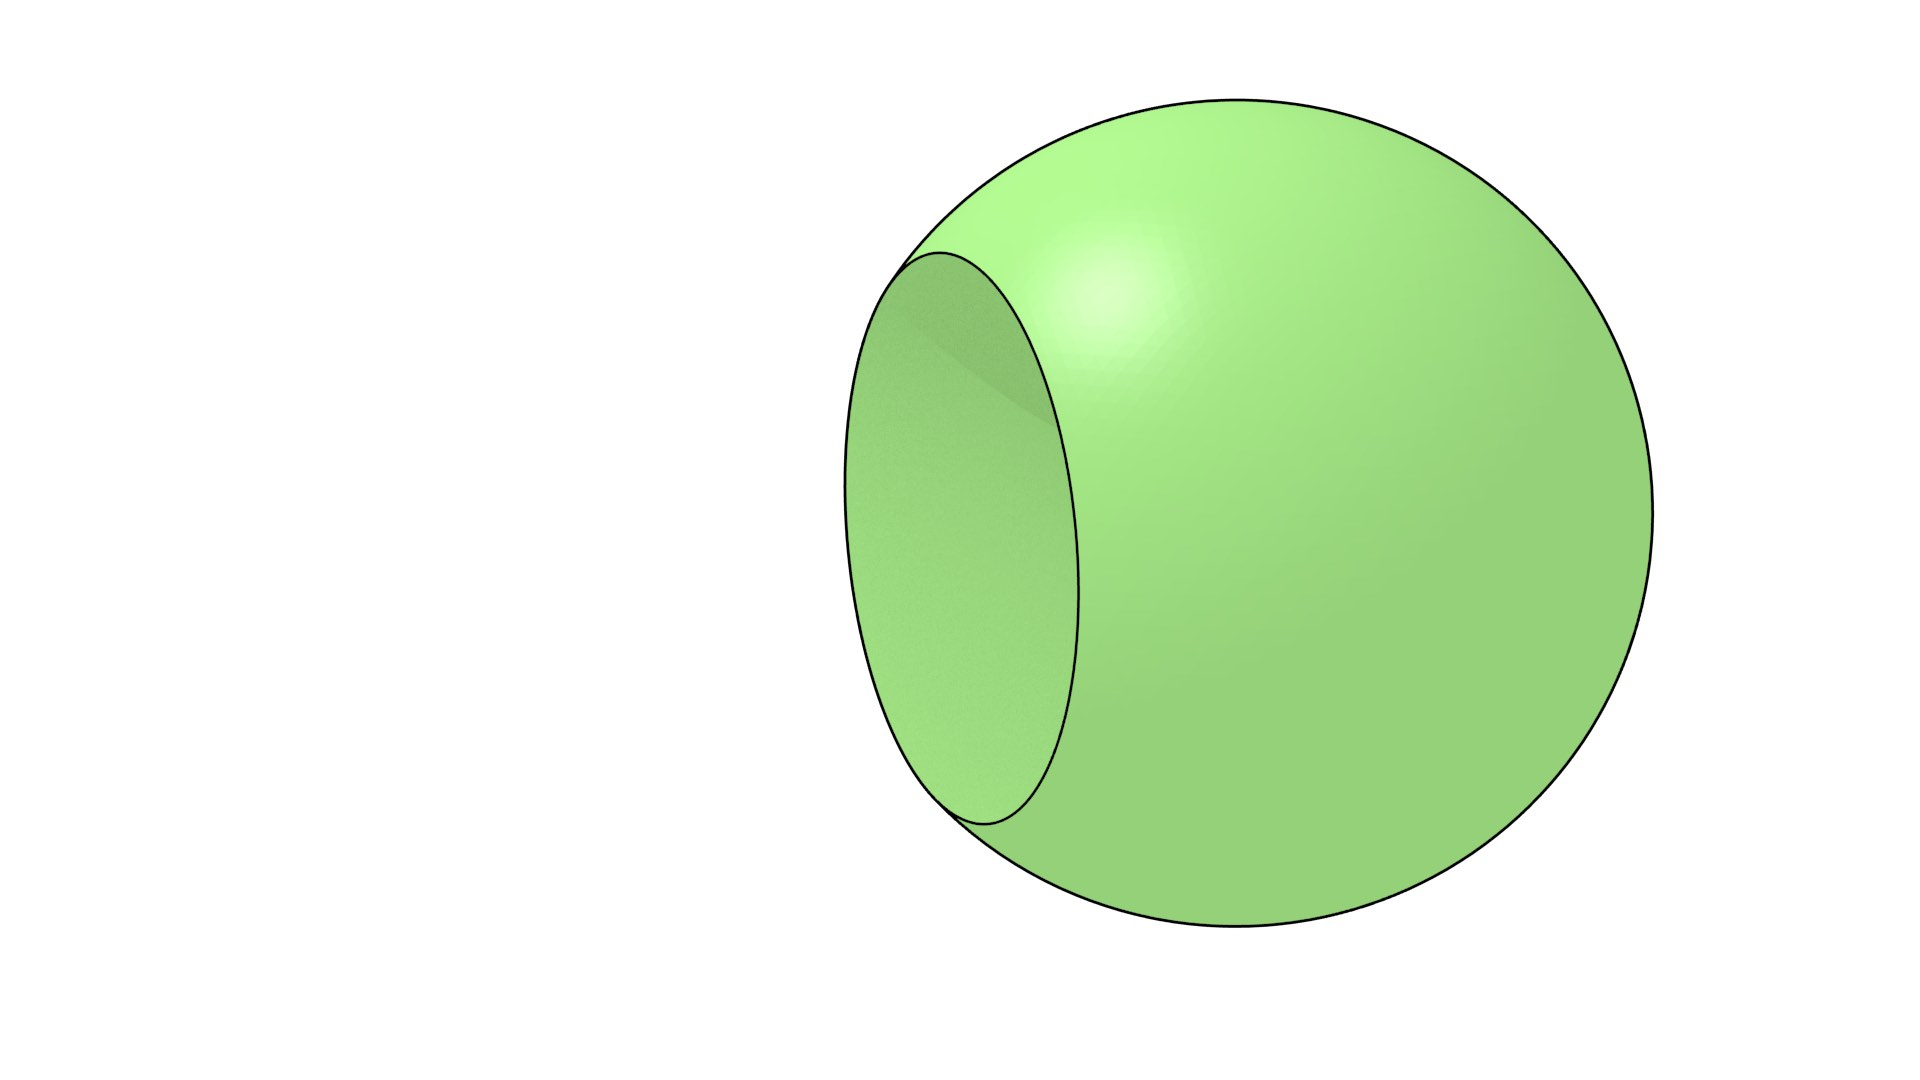
\includegraphics[width=\linewidth]{figs/boolean-difference}
\caption{}%
\label{subfig:boolean-difference}
\end{subfigure}
\caption{Based on (a) two balls \(\mathbb{A}\) and \(\mathbb{B}\), other objects can be defined using Boolean set operations, such as: (b) the intersection \(\mathbb{A} \cap \mathbb{B}\), (c) the union \(\mathbb{A} \cup \mathbb{B}\), and (d) the difference \(\mathbb{A} - \mathbb{B}\).}%
\label{fig:boolean}
\end{figure}

Boolean point set operations are based on the Boolean operations on sets, which are mainly:

\begin{description}
\item[union] of\marginnote{union}\index{union} the sets \(\mathbb{A}\) and \(\mathbb{B}\), denoted as \(\mathbb{A} \cup \mathbb{B}\), is the set containing the elements that are in \(\mathbb{A}\) or \(\mathbb{B}\), \ie\ \( \mathbb{A} \cup \mathbb{B} = \left\{ x : x \in \mathbb{A} \vee x \in \mathbb{B} \right\} \);
\item[intersection] of\marginnote{intersection}\index{intersection} the sets \(\mathbb{A}\) and \(\mathbb{B}\), denoted as \(\mathbb{A} \cap \mathbb{B}\), is the set containing the elements that are in both \(\mathbb{A}\) and \(\mathbb{B}\), \ie\ \( \mathbb{A} \cap \mathbb{B} = \left\{ x : x \in \mathbb{A} \wedge x \in \mathbb{B} \right\} \);
\item[set difference] of\marginnote{difference}\index{difference} the sets \(\mathbb{A}\) and \(\mathbb{B}\), denoted as \(\mathbb{A} - \mathbb{B}\) or \(\mathbb{A} \setminus \mathbb{B}\), is the set containing the elements that are in \(\mathbb{A}\) but not in \(\mathbb{B}\), \ie\ \( \mathbb{A} - \mathbb{B} = \left\{ x : x \in \mathbb{A} \wedge x \notin \mathbb{B} \right\} \);
\item[symmetric difference] of\marginnote{symmetric difference}\index{symmetric difference} the sets \(\mathbb{A}\) and \(\mathbb{B}\), denoted as \(\mathbb{A} \triangle \mathbb{B}\), \(\mathbb{A} \ominus \mathbb{B}\) or \(\mathbb{A} \oplus \mathbb{B}\), is the set containing the elements that are either in \(\mathbb{A}\) or in \(\mathbb{B}\) but not in both, \ie\ \( \mathbb{A} \triangle \mathbb{B} = \left\{ x : x \in \mathbb{A} - \mathbb{B} \cup \mathbb{B} - \mathbb{A} \right\} \).
\end{description}

The key point about these operations is that they do not need to perform any geometric computations, since it is possible to tell if an element (\ie\ point) is in the new point set by just checking whether it is in its children's point sets.
It is thus trivially easy to do Boolean point set operations on individual points.

Based on this knowledge, we could build a crude CSG implementation directly on a point cloud or voxel grid by: (i) for each leaf node, checking whether each point/voxel meets the point set definition in the node, and (ii) for each non-leaf node, applying the Boolean set operations on the point sets represented by its child nodes point by point.
However, since this easy solution is not applicable to other data models, we will look at a better solution that works better in practice.

\section{Nef polyhedra}

\emph{Nef polyhedra}\marginnote{Nef polyhedra}\index{Nef polyhedra}, named after Walter Nef, are an alternative representation of polygons and polyhedra (\ie\ not the usual b-rep meshes) that is based on the concept of a \emph{local pyramid}, which is a structure that stores the neighbourhood information around every vertex (\reffig{nef}).
Polygons and polyhedra can be stored as a set of local pyramids and their location (as a set of 2D/3D coordinates).

\begin{figure}
\centering
\begin{subfigure}[b]{0.5\linewidth}
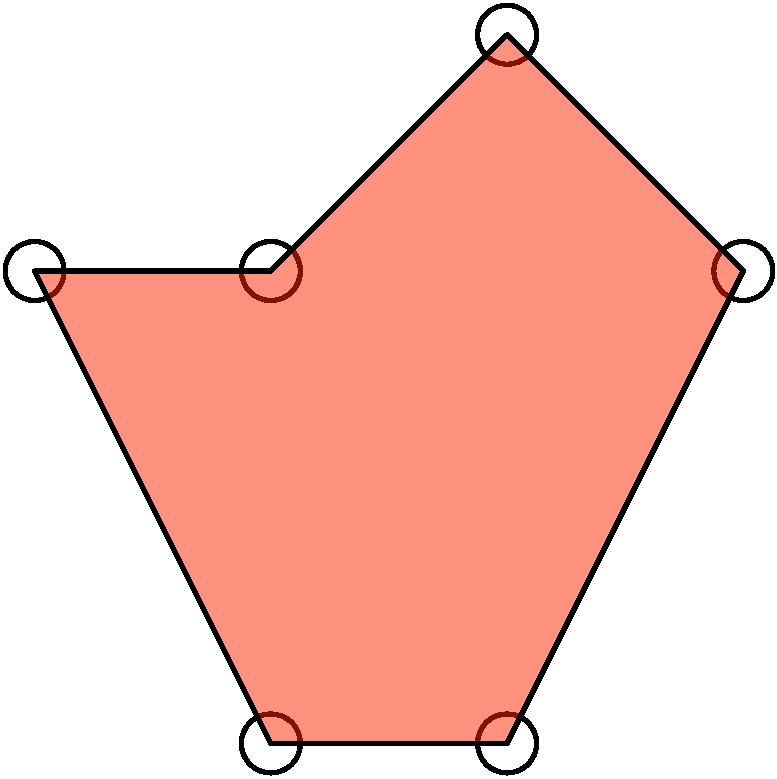
\includegraphics[width=\linewidth]{figs/nef-1}
\caption{}%
\end{subfigure}
\begin{subfigure}[b]{0.35\linewidth}
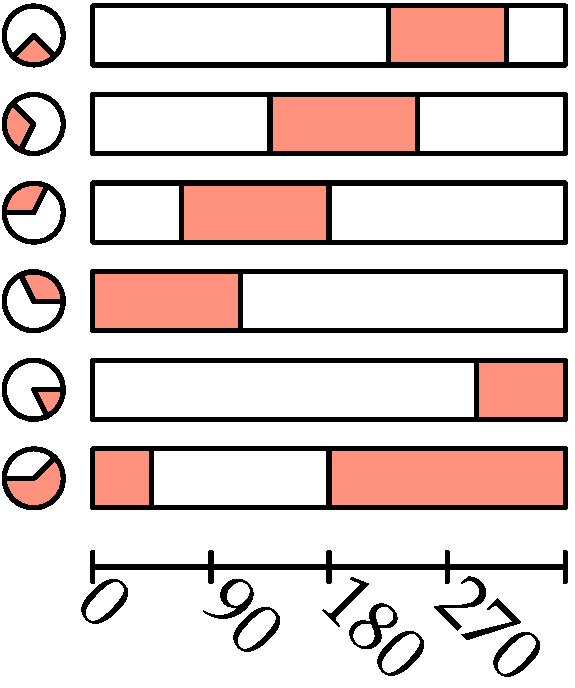
\includegraphics[width=\linewidth]{figs/nef-2}
\caption{}%
\end{subfigure}
\caption{(a) A Nef polygon is represented indirectly as (b) a set of local pyramids (circles).
At every local pyramid, the polygon (red) becomes an angular interval.
Incident edges become points at the endpoints of these intervals.}%
\label{fig:nef}
\end{figure}

\subsection{Local pyramids}

The local pyramid\marginnote{local pyramid}\index{local pyramid} of a vertex contains the intersection of an infinitesimally small sphere (in 3D) or circle (in 2D) with the volumes, faces and edges incident to this vertex.
An incident volume thus becomes a face, an incident face becomes an edge, and an incident edge becomes a vertex on the surface of the local pyramid sphere/circle, essentially lowering the dimension of every object by one (just like boundary representation does!).

The key thing to understand here is the following: \emph{a 2D/3D object represented as a set of local pyramids (and their location) can individually be stored using 1D/2D data structures}.
This is a process akin to boundary representation, but it does not have problems with non-manifold objects (unlike boundary representation).

In practice, computing the local pyramid at a local vertex is also a relatively simple operation.
We will not go through the details here (see the references in the notes if you are interested), but in 2D, it involves computing the angle of its neighbouring vertices as you rotate around the vertex, and marking the intervals between these vertices with the polygons that you pass through while doing so.
In 3D, it is a more complex operation involving the computation of an arrangement of lines in a spherical coordinate system, and the location of every neighbouring vertex is defined by two angles (rather than one).

\subsection{Computing Boolean point set operations on Nef polyhedra}

Boolean point set operations on Nef polyhedra (and many other geometric operations) can be computed in three steps: subdivision, selection and simplification.
This is a common scheme used in geometric computing in general, and we will discuss what each of these involves in this specific case.

\begin{description}

\item[Subdivision] involves\marginnote{subdivision}\index{subdivision} computing an overlay of the input polyhedra, thus creating the overall structure where the result will be put (\ie\ the vertices, edges, faces and volumes).

In 2D, this is also a computation of a line arrangement (also known in GIS as map overlay), where the output is a set of vertices and edges representing all the input lines of both polygons, but where edges do not intersect except at their common vertex end points.
Vertices (\ie\ local pyramids) will be located at the position of all input vertices and at every new intersection between lines.

In 3D, it is a similar operation, but the new vertices (\ie\ local pyramids) are located at line-polygon intersections as well.
These can be calculated by computing a plane passing through the polygon and intersecting it with the line.

\item[Selection] involves\marginnote{selection}\index{selection} checking whether each face (in 2D) or volume (3D) should be part of the output or not, marking it as such in the relevant parts of the local pyramids.
This is done by testing whether it is in the interior or exterior of the input Nef polygons/polyhedra.

\item[Simplification] involves\marginnote{simplification}\index{simplification} removing unnecessary structures in a way that does not alter the point set that is represented, which is akin to the dissolving operations common in GIS\@.
This is done by deleting local pyramids when they do not actually represent a new vertex, or when are not subdivided.

\end{description}

\reffig{nef-boolean} shows an example of how this works in practice in 2D.
A 2D Boolean point set operation starts from two Nef polygons \(A = (g, b, f, i)\) and \(B = (a, f, k, j, e, c)\)---each of which is stored as a set of local pyramids at its corresponding vertices.
As shown previously in \reffig{nef}, each of these 2D local pyramids can be stored as a list of 1D intervals, \eg\ at vertex \(a\), polygon \(B = [225, 315]\), where the values are in degrees.

The operation first computes the intersections between the line segments (as an overlay problem), creating the new vertices \(d\) and \(h\).
The location of these vertices can be calculated using the equations of the corresponding lines.
The vertices of each polygon and the intersection points between the line segments yield the local pyramids to be considered.

Then, the local pyramid intervals for both polygons at all of these locations are computed.
For instance, at vertex \(a\), \(A = \emptyset{}\) and \(B = [225, 315]\).
A Boolean set operation is then computed by applying it to the local pyramids (\ie\ to the intervals).
For instance, at vertex \(a\), \(\neg A = \mathbb{U} = [0, 360]\) and \(\neg B = [315, 225]\) (by inverting the range), \(A \cup B = [225, 315]\) (by combining the ranges), \(A \cap B = \emptyset{}\) (by finding common parts of the ranges), and \(A - B = \emptyset{}\) (by removing from the ranges of \(A\) those of \(B\)).

Finally, unnecessary local pyramids can be removed from the output: \(f\) in \(A \cup B\); \(a\), \(b\), \(c\), \(g\), \(i\), \(j\) and \(k\) in \(A \cap B\); and \(a\), \(c\), \(j\) and \(k\) in \(A - B\).

\begin{figure}
\centering
\begin{subfigure}[b]{0.23\linewidth}
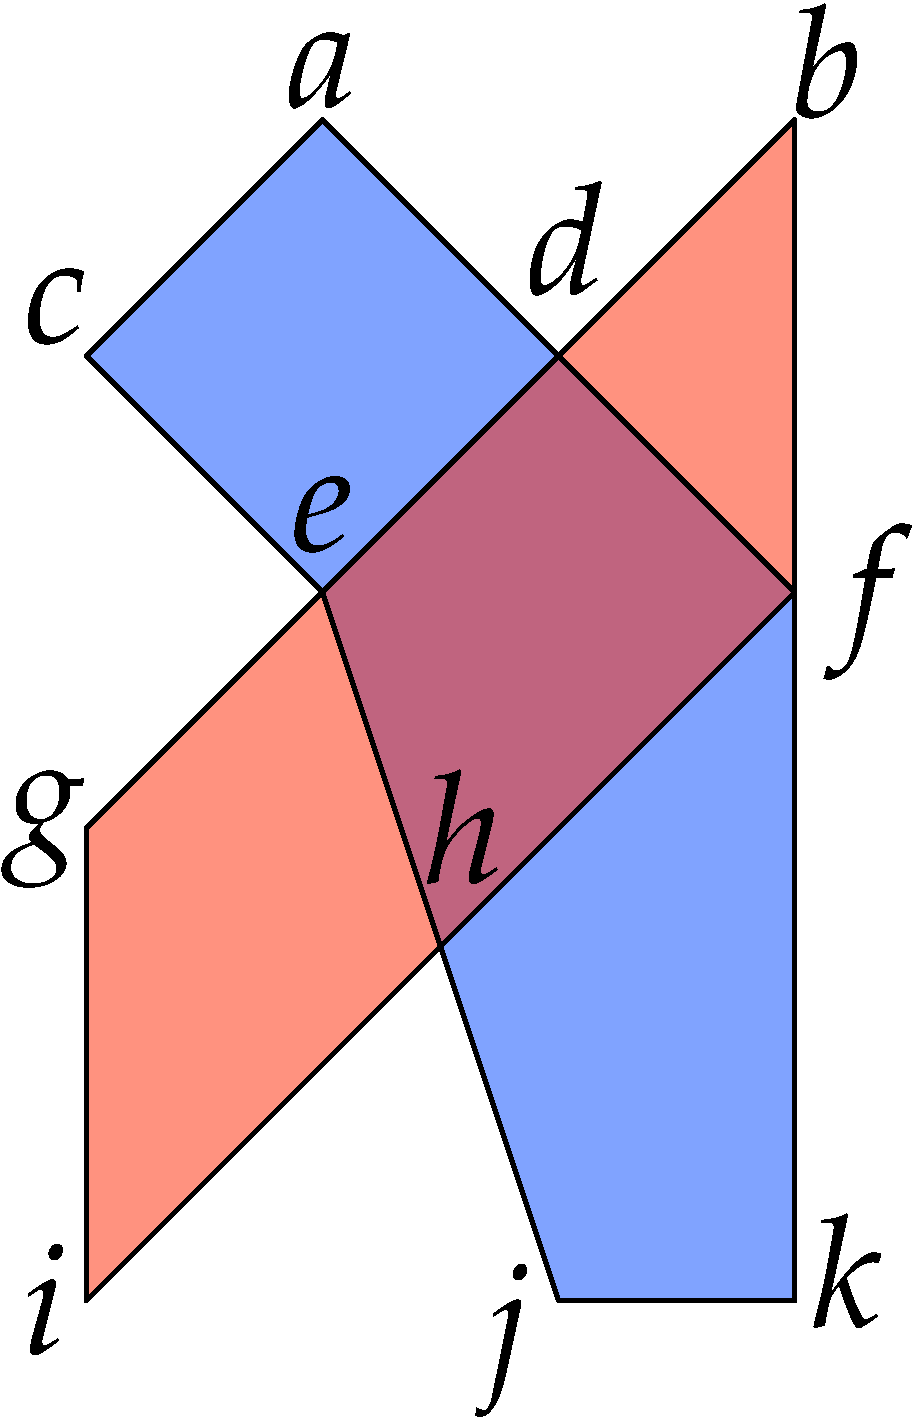
\includegraphics[width=\linewidth]{figs/nef-boolean-1}
\caption{}%
\end{subfigure}
\quad
\begin{subfigure}[b]{0.6\linewidth}
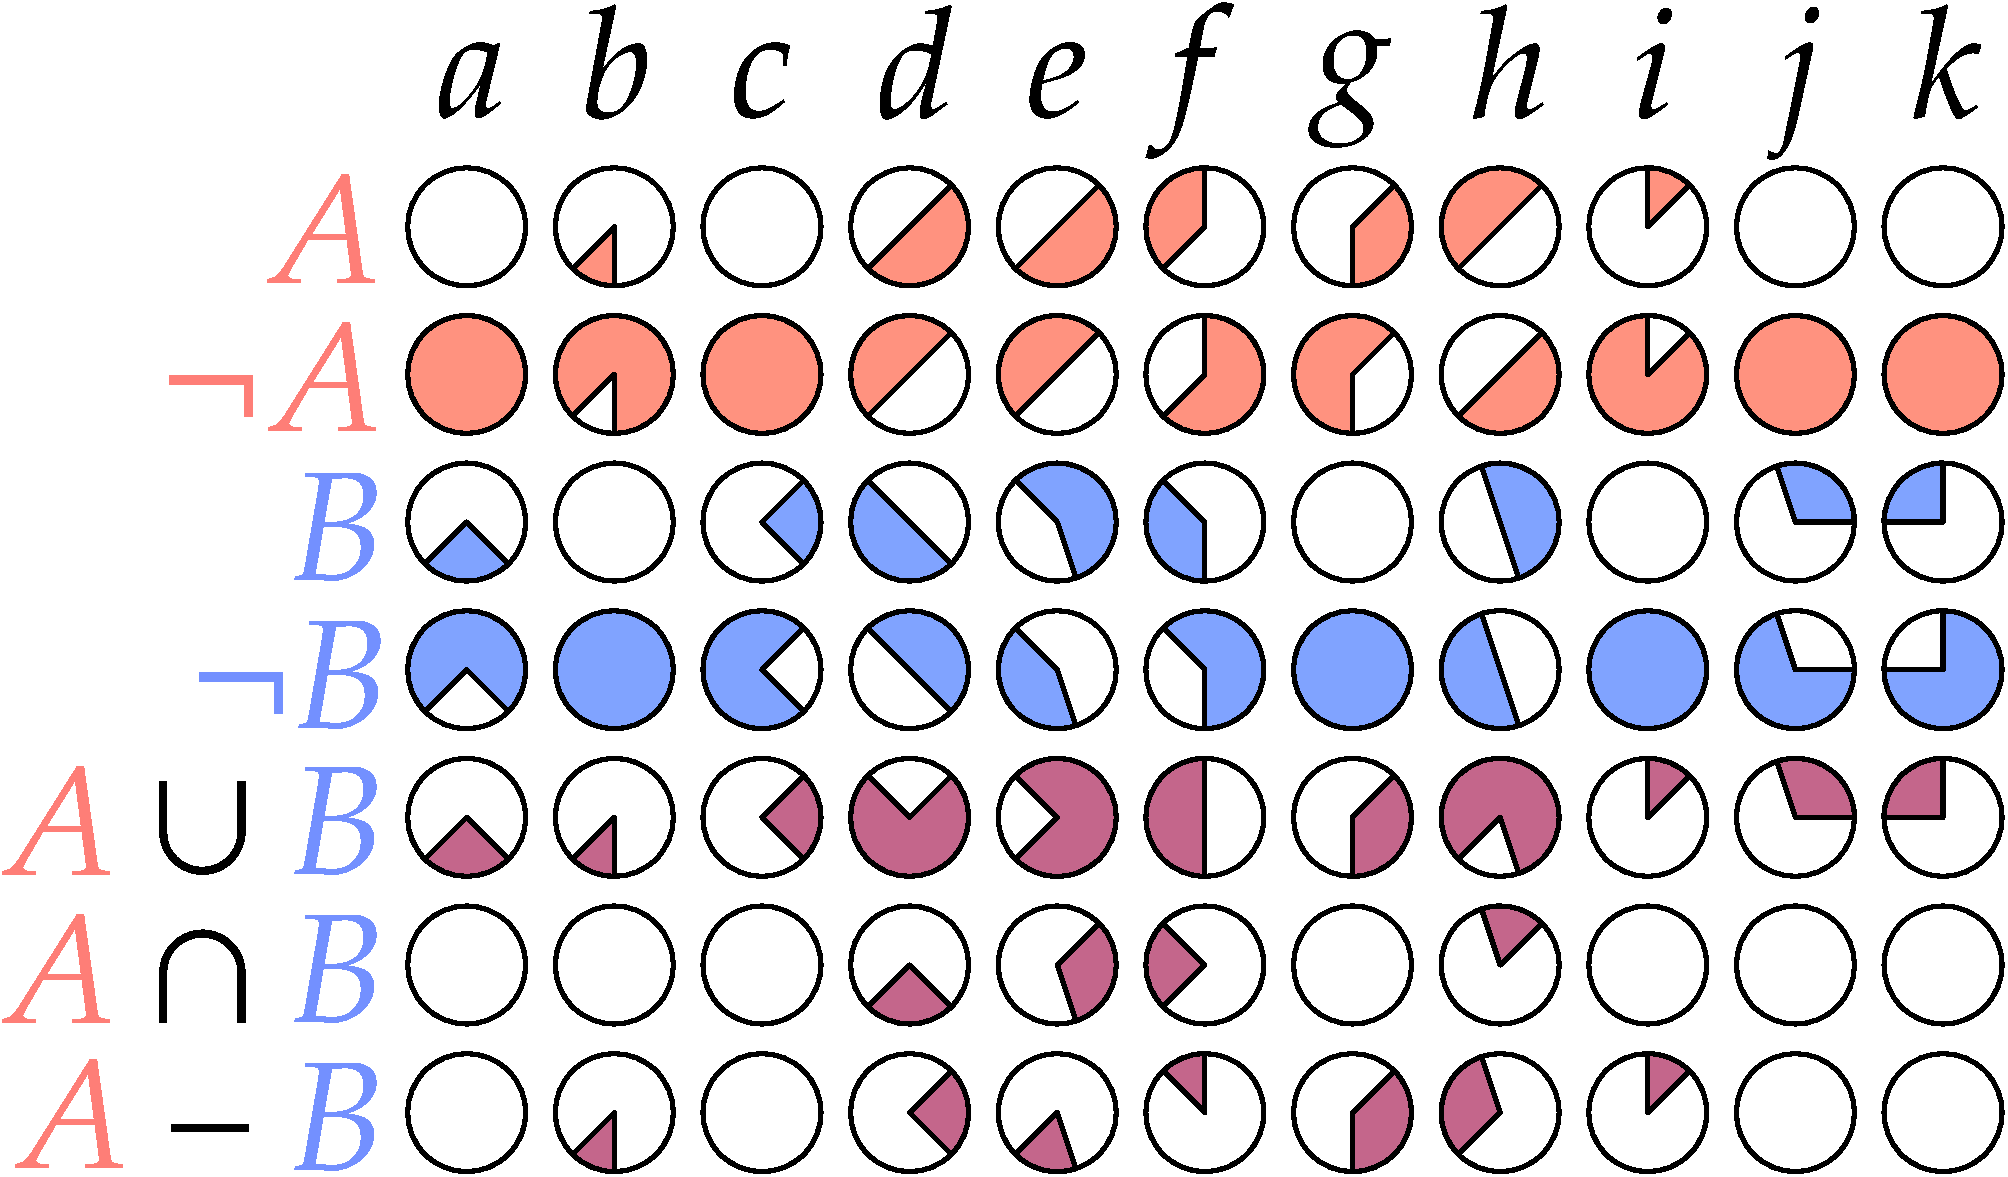
\includegraphics[width=\linewidth]{figs/nef-boolean-2}
\caption{}%
\end{subfigure}
\caption{Various Boolean point set operations on (a) the Nef polygons \(A\) (red) and \(B\) (blue) that can be performed on (b) their local pyramids.}%
\label{fig:nef-boolean}
\end{figure}

\subsection{3D Nef polyhedra in practice: selective Nef complexes}

3D Nef polyhedra and Boolean point set operations on them can be implemented using different data structures, but an excellent open implementation (see notes) uses a data structure called \emph{selective Nef complexes}\marginnote{selective Nef complex}\index{selective Nef complex} (\reffig{snc}).

\begin{figure}
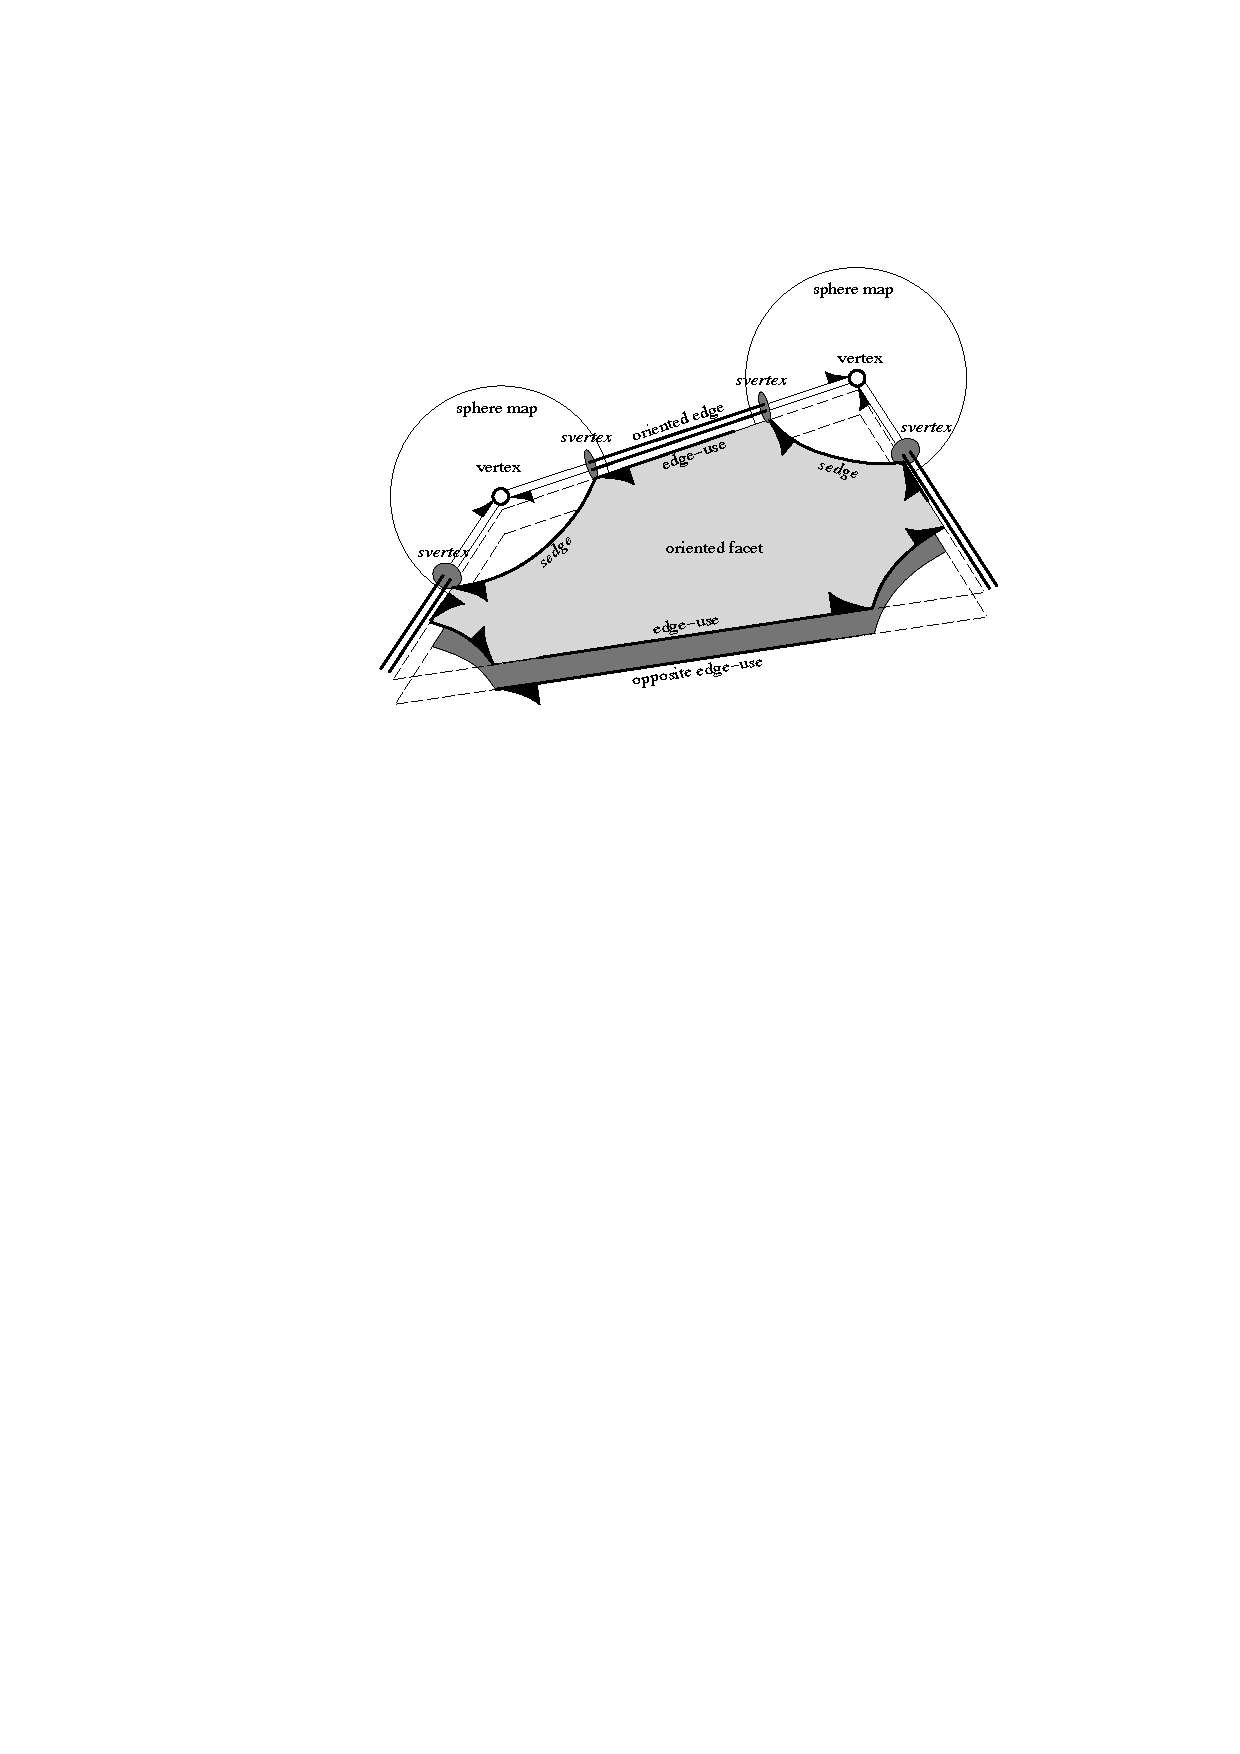
\includegraphics[width=\linewidth]{figs/snc}
\caption{A selective Nef complex.
The standard half-edge structure on 3D space uses faces (as an oriented facet for each incident polyhedron), edges (as an edge-use for each incident oriented facet) and vertices.
The half-edge structure on the surfaces of the spheres representing local vertices, known as sphere maps, uses \emph{sfaces} (per incident polyhedron but not shown here), \emph{sedges} (per incident face) and \emph{svertices} (per incident edge).
From \citet{Hachenberger06}.}%
\label{fig:snc}
\end{figure}

Selective Nef complexes (SNC) use a combination of two half-edge data structures:

\begin{itemize}
\item a standard half-edge data structure on 3D space, which stores each face of each polyhedron as a cycle of \emph{edge-uses} connecting vertices;
\item a half-edge data structure to represent each local pyramid (one per vertex) as a subdivision on the surface of an (infinitesimally small) sphere.
\end{itemize}

Each vertex is linked to its sphere map, where each incident volume corresponds to a face on its sphere map (sface), each incident face corresponds to an edge (sedge), and each incident edge corresponds to a vertex (svertex).
These corresponding elements are linked to each other, which makes it possible to navigate both on the half-edge data structure in 3D space (\eg\ by going from an edge-use to the next to cycle around a face) and on the half-edge data structure of a sphere map (\eg\ by going from one sedge to the next to cycle around an sface).

%%%
%
\section{Exercises}

\begin{enumerate}
	\item How can you define a cube using:
	\begin{enumerate}
		\item a parametric representation
		\item a b-rep data structure
		\item an intersection of half-spaces
	\end{enumerate}
	\item In the line \(L = a p_1 + (1-a) p_2 \), what is the geometry given by \(a < 0\) and \(a > 1\)?
	\item Compute the ranges for the local pyramids of some other vertices in 
	\reffig{nef-boolean}.
	\item In which cases is simplification needed in 2D\@?
	\item Imagine the voxel CSG engine briefly mention in \refsec{psetops}. What would you use for leaf nodes in the CSG tree? How would you implement Boolean set operations on them?
\end{enumerate}



%%%
%
\section{Notes and comments}

If you need more help with the mathematical background, check the Wikipedia pages on sets\footnote{\url{https://en.wikipedia.org/wiki/Set_(mathematics)}}, set algebra\footnote{\url{https://en.wikipedia.org/wiki/Algebra_of_sets}}.

The earliest description of CSG is likely \citet[\S{}12.3]{Requicha77} and its properties is \citet{Requicha78}.
However, it is more of a culmination of efforts of many people.
For instance, \citet{Shamos76} and \citet{Preparata79} show that it is possible to represent any convex object (of any dimension) as the intersection of a finite number of half-spaces.
In order to see how such a decomposition can be done, see \citet{Chazelle79} or \citet{Bajaj90}.
A nice example of how half-spaces can be stored in practice is \citet{Naylor90}.

Nef polyhedra were originally described in \citet{Nef78}, although a much better description including the way they work with Boolean set operations is available in \citet{Bieri88}.

For more background on the line arrangement problem, see the relevant Wikipedia page\footnote{\url{https://en.wikipedia.org/wiki/Arrangement_of_lines}}.
For a clear description of how to compute one, see \citet[\S{}2]{deBerg08} or the user manual of the \texttt{Arrangements\_2} package of CGAL\footnote{\url{https://doc.cgal.org/latest/Arrangement_on_surface_2/index.html}}.

Nef polyhedra as a CSG engine in practice is only possible thanks to \citet{Seel01} in 2D and \citet{Hachenberger06} in 3D.
They discuss how to compute local pyramids in 2D and 3D, as well as Boolean point set operations on polygons and polyhedra.
They are implemented in the CGAL packages 2D Boolean Operations on Nef Polygons\footnote{\url{https://doc.cgal.org/latest/Nef_2/index.html}} and 3D Boolean Operations on Nef Polyhedra\footnote{\url{https://doc.cgal.org/latest/Nef_3/index.html}}.

The general scheme to perform geometric operations in three steps (subdivision, selection and simplification) is discussed by \citet{Rossignac89}.
